% Customizable fields and text areas start with % >> below.
% Lines starting with the comment character (%) are normally removed before release outside the collaboration, but not those comments ending lines

%%%%%%%%%%%%% local definitions %%%%%%%%%%%%%%%%%%%%%


%%%%%%%%%%%%%%%  Title page %%%%%%%%%%%%%%%%%%%%%%%%
\cmsNoteHeader{AN-20-200}
% >> Title: please make sure that the non-TeX equivalent is in PDFTitle below for papers. For PASs, PDFTitle can be used with plain TeX.
\title{Search for WZ Resonances into the $\ell\ell\ell\nu$ final state at 13TeV using the full RunII dataset}

% >> Authors
%Author is always "The CMS Collaboration" for PAS and papers, so author, etc, below will be ignored in those cases
%For multiple affiliations, create an address entry for the combination
%To mark authors as primary, use the \author* form
\address[inst1]{Catholic University of America (US)}
\author*[inst1]{Rachel Bartek}
\author*[inst1]{Aaron Dominguez}
\author*[inst1]{Rishabh Uniyal}
\author*[inst1]{Andres Vargas Hernandez}


% >> Date
% The date is in yyyy/mm/dd format. Today has been
% redefined to match, but if the date needs to be fixed, please write it in this fashion.
\date{\today}

% >> Abstract
% Abstract processing:
% 1. **DO NOT use \include or \input** to include the abstract: our abstract extractor will not search through other files than this one.
% 2. **DO NOT use %**                  to comment out sections of the abstract: the extractor will still grab those lines (and they won't be comments any longer!).
% 3. For PASs: **DO NOT use CMS tex macros.**...in the abstract: CDS MathJax processor used on the abstract doesn't understand them _and_ will only look within $$. The abstracts for papers are hand formatted so macros are okay.
\abstract{
 A search for narrow-width resonances decaying to a pair of vector bosons WZ which themselves
 decay to three electrons(muons) and missing energy using $137.4 fb^{-1}$ of data
 recorded by the CMS detector in $pp$ collisions at a center of mass energy of
 $\sqrt{s}= 13$ TeV is presented.

 No significant deviation from Standard model prediction is observed. 
}

% >> PDF Metadata
% Do not comment out the following hypersetup lines (metadata). They will disappear in NODRAFT mode and are needed by CDS.
% Also: make sure that the values of the metadata items are sensible and are in plain text with the possible exception of the PDFtitle for a PAS. Then you can use pure TeX symbols as if on a typewriter. Examples: $\sqrt{s}=13\TeV$ => $sqrt{s}=$ 13 TeV; 32\fbinv => 32 fb$^{-1}$
% No unescaped comment % characters.
% No curly braces {} except for TeX in the PDFtitle.
\hypersetup{%
pdfauthor={Andres Vargas Hernandez},%
pdftitle={Search for WZ Resonances into the ellellellnu final state at 13TeV using the full RunII dataset},%
pdfsubject={CMS},%
pdfkeywords={CMS, your topics}}

\maketitle %maketitle comes after all the front information has been supplied
% >> Text
%%%%%%%%%%%%%%%%%%%%%%%%%%%%%%%%  Begin text %%%%%%%%%%%%%%%%%%%%%%%%%%%%%
%% **DO NOT REMOVE THE BIBLIOGRAPHY** which is located before the appendix.
%% You can take the text between here and the bibiliography as an example which you should replace with the actual text of your document.
%% If you include other TeX files, be sure to use "\input{filename}" rather than "\input filename".
%% The latter works for you, but our parser looks for the braces and will break when uploading the document.
%%%%%%%%%%%%%%%

% >> acknowledgments (for journal papers only)
% The latest version of the acknowledgments will be included from https://twiki.cern.ch/twiki/bin/viewauth/CMS/Internal/PubAcknow as of the date of submission. 
% !!! Anything you supply here WILL BE OVERWRITTEN, but you can include the current text as an example.
%
% Modify to match either US or UK English spelling for centre/center, programme/program. For PRL use the short version, for JINST normally use the long version. All others take the middle length version other than exceptional cases.
\begin{acknowledgments}
\end{acknowledgments}

\section{Introduction}

The succesful finding of the, widely expected, Higgs Boson ~\cite{higgsPaperCMS,higgsPaperATLAS}
(the only scalar fundamental particle), and its 125 GeV, ligther than expected mass,
requires a high level fine tuning of the Standard Model (SM) through the
manually set properties of the now seventeen elementary particles.
This suggests an underlaying, more fundamental structure to be discovered and
a theory beyond the standard model. Other
reasons that are strongly coherent with this suggestion are: the wildly
different masses of the three different families of particles, the lack of
mass ratios predictions, open questions such as the structure of dark matter,
let alone the inclusion of gravity.

Some of the most promising hypotheses addressing the Electroweak Symmetry
Breaking (EWSB), propose that the Higgs field
emerges from a new strongly-interacting composite sector. An unavoidable
consequence from these theories, is the existance of Spin-1 vector resonances
decaying to heavy vector bosons.  Broadly speaking these resonances
fall into  two categories: electrically
charged resonances, commonly refered as $W^{\prime}$ and
neutral resonances $Z^{\prime}$. These resonances might be available at the TeV
scale ~\cite{tevscale2014}, the current LHC energy range. The question then becomes:
can experimental evidence of the existance of such resonances be found?

Vector boson resonances are a prediction of a large number
of SM extensions, including, but not limited to, the Electroweak Chiral
Lagrangian model ~\cite{echl2017}, the Little Higgs
~\cite{littlehiggs2007}, the Randall-Subdrum  model ~\cite{randall1999}, the
Minimal walking technicolor ~\cite{technicolor2007}, or models where the Higgs
is a composite pseudo-Nambu-Goldstone boson ~\cite{composite2016}.

\begin{figure}[tph]
  \centering
  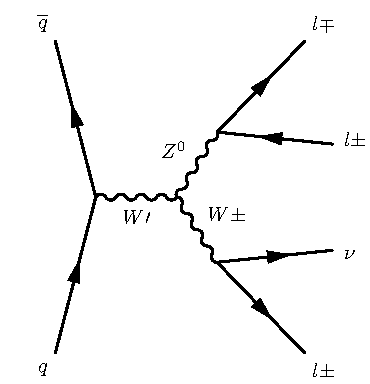
\includegraphics[width=0.4\textwidth]{fig/WprimeFeynmanDiagram.pdf}
  \caption{ Feynman Diagram of the decay for the
    electrically charged WZ resonance $W^{\prime}$}
  \label{fig:Wprime_FeynmanDiagram}
\end{figure}

In this analysis, we test a set of theoretical models based on a phenomenological
lagrangian that contains Heavy Vector Triplets (HVT): the HVT framework, which
generalizes a large number of models predicting Spin-1 resonances ~\cite{hvt2014}.
Using two benchmarks: A weakly coupled extended gauge symmetry (referred as model A) and a
strongly coupled composite higgs scenario (model B). Further theoretical treatment of these models
is provided by Refs. ~\cite{hvt2014,modelA1980,modelB2011}. Specifically, a search
for an electrically charged resonance $W^{\prime}$ is performed. This search focuses
on the $W^{\prime}$ fully leptonic decay:
$W^{\prime}\rightarrow WZ \rightarrow \ell\nu \ell\ell$ ($\ell = e$ or $\mu$).
Despite the low branching ratio of the leptonic decay, it offers low SM backgrounds and high
sensitivity in the low mass resonance range. In this channel, the SM $Z^{0}$
boson decays to a pair of same flavoured, opposite charged leptons and the
electrically charged $W^{\pm}$ decays to a lepton and a neutrino, see Feynman diagram
on figure \ref{fig:Wprime_FeynmanDiagram}. The neutrino $\nu$ escapes
undetected and therefore needs to be reconstructed from the missing transverse
energy in the Compact Muon Solenoid (CMS) detector.

Initial studies look for an enhancement of the Signal/Background ratio,
based on the kinematic variables to find regions in the phase-space sensitive
to the presence of the signal; these include studies on the performance of
the High Level Trigger, different options of lepton identification, isolation,
and other detector-specific requirements.

The accuracy of the MC simulations for the SM processes is then studied in a
dedicated signal-depleted control region of the phase space. A variety of
corrections on the MC samples are applied in order to account for the different
rates of efficiencies in the data reconstruction, particle identification, and
inefficiencies in the simulation of generated processes, as well as the
contribution from multiple proton-to-proton interactions occurring per bunch
crossing at the LHC accelerator.

The spectrum of the invariant mass for the diboson resonance candidates is
examined where a localized excess of events is expected if the resonance is
found, or otherwise, an agreement with the rates predicted by the standard model
within the statistical and systematic uncertainties will be found.
A fit to a background-only and background plus signal hypothesis is performed
through maximum likelihood estimation. Systematic uncertainties effects are
treated as nuisance parameters of the likelihood function.

The analysis is based on proton-proton collision data, with a center of mass
energy of $\sqrt{s}=13$ TeV collected by the CMS collaboration during the the
2016-2018 period, corresponding to an integrated luminosity of $L=137.2~fb^{-1}$.


\section{Search Strategy}


\section{Data and Montecarlo Samples}

\subsection{Data}


\begin{table}[h]
\centering
\caption{List of datasets used in the analysis.}
\begin{tabular}{|l|l|l|l|}
\hline
Year & Dataset & Run & Version \\ \hline
2016 & SingleMuon     & B           & ver2-v1 \\
     &                & C,D,E,F,G,H & v1      \\
     & SingleElectron & B           & ver2-v1 \\
     &                & C,D,E,F,G,H & v1      \\
     & SinglePhoton   & B           & ver2-v1 \\
     &                & C,D,E,F,G,H & v1      \\ \hline
2017 & SingleMuon     & B,C,D,E,F & v1 \\
     & SingleElectron & B,C,D,E,F & v1 \\
     & SinglePhoton   & B,C,D,E,F & v1 \\\hline
2018 & SingleMuon & A,B,C,D & v1 \\
     & EGamma     & A,B,C,D & v1 \\ \hline
\end{tabular}
\label{tab:Datasets}
\end{table}

\begin{table}[htbp]
  \footnotesize
  \topcaption{
    The golden JSON files
  }
  \centering
  \label{tab:gJSON}
  \begin{tabular}{ c l }
    \hline
    Year & File \\
    \hline
    2016 & Cert\_271036-284044\_13TeV\_ReReco\_07Aug2017\_Collisions16\_JSON.txt \\
    2017 & Cert\_294927-306462\_13TeV\_PromptReco\_Collisions17\_JSON.txt \\
    2018 & Cert\_314472-325175\_13TeV\_PromptReco\_Collisions18\_JSON.txt \\
    \hline
  \end{tabular}
\end{table}


\subsection{Montecarlo Samples}


\begin{sidewaystable}[htb]
\begin{center}
\caption{List of background samples for 2016}
\footnotesize
\begin{tabular}{|l|l|l|l|}
\hline
Background  & Sample & XSec [pb] & Comment \\ \hline
DY          & DYJetsToLL\_M-10to50\_TuneCUETP8M1\_13TeV-amcatnloFXFX-pythia8      & 18610.0 & For low di-lepton mass \\ % DYJetsToLL_M-10to50_ext1
Top         & TTTo2L2Nu\_TuneCUETP8M2\_ttHtranche3\_13TeV-powheg-pythia8          & 87.310 & \\ % TTTo2L2Nu
& ST\_tW\_antitop\_5f\_inclusiveDecays\_13TeV-powheg-pythia8\_TuneCUETP8M1        & 35.60 & \_ext1 \\ \hline % ST_tW_antitop
\end{tabular}
\label{tab:BkgList1}
\end{center}
\end{sidewaystable}





\section{Uncertainties}


\section{Object definitions and Event selection}


\section{Corrections on MC}


\section{Results}





%% **DO NOT REMOVE BIBLIOGRAPHY**
\bibliography{auto_generated}
%% examples of appendices.
%\clearpage
%\appendix
%\section{Appendix name}
%%% DO NOT ADD \end{document}!

